
\documentclass[sigconf]{acmart}

\usepackage{graphicx}
\usepackage{booktabs}
\usepackage{hyperref}
\usepackage{subcaption}
\usepackage{listings}

\title{A Proxy Persona Tool For Web Viewing and Chat Interaction}

\author{Christopher B. Rauch}
\affiliation{%
  \institution{Drexel University}
  \city{Philadelphia}
  \state{PA}
  \country{USA}
}
\email{cr625@drexel.edu}

\author{Hyung Wook Choi}
\affiliation{%
  \institution{Drexel University}
  \city{Philadelphia}
  \state{PA}
  \country{USA}
}
\email{hc685@drexel.edu}

\author{Michael L. Nelson}
\affiliation{%
  \institution{Old Dominion University}
  \city{Norfolk}
  \state{VA}
  \country{USA}
}
\email{mln@cs.odu.edu}

\author{Alex H. Poole}
\affiliation{%
  \institution{Drexel University}
  \city{Philadelphia}
  \state{PA}
  \country{USA}
}
\email{ahp56@drexel.edu}

\author{Travis Reid}
\affiliation{%
  \institution{Old Dominion University}
  \city{Norfolk}
  \state{VA}
  \country{USA}
}
\email{treid003@odu.edu}

\author{Michele C. Weigle}
\affiliation{%
  \institution{Old Dominion University}
  \city{Norfolk}
  \state{VA}
  \country{USA}
}
\email{mweigle@cs.odu.edu}

\author{Mat Kelly}
\affiliation{%
  \institution{Drexel University}
  \city{Philadelphia}
  \state{PA}
  \country{USA}
}
\email{mkelly@drexel.edu}

\begin{abstract}
This demo presents A-Proxy, an interactive proxy tool designed to capture, inspect, and preserve personalized online activity in real-time browsing sessions from the context of specific personas. The tool enables archivists to save these browsing sessions as user journeys related to specific topics. The archived data offers a more persistent storage option for recorded behaviors and the opportunity to examine personalization aspects in a consistent way. We intend to extend the current functionality to leverage personalization options available in large language models (LLMs) and allow persona information to be passed as additional context to these models.
\end{abstract}

\keywords{web archiving, advertisements, proxy server, personalization}

\begin{document}
\begin{teaserfigure}
  \centering
  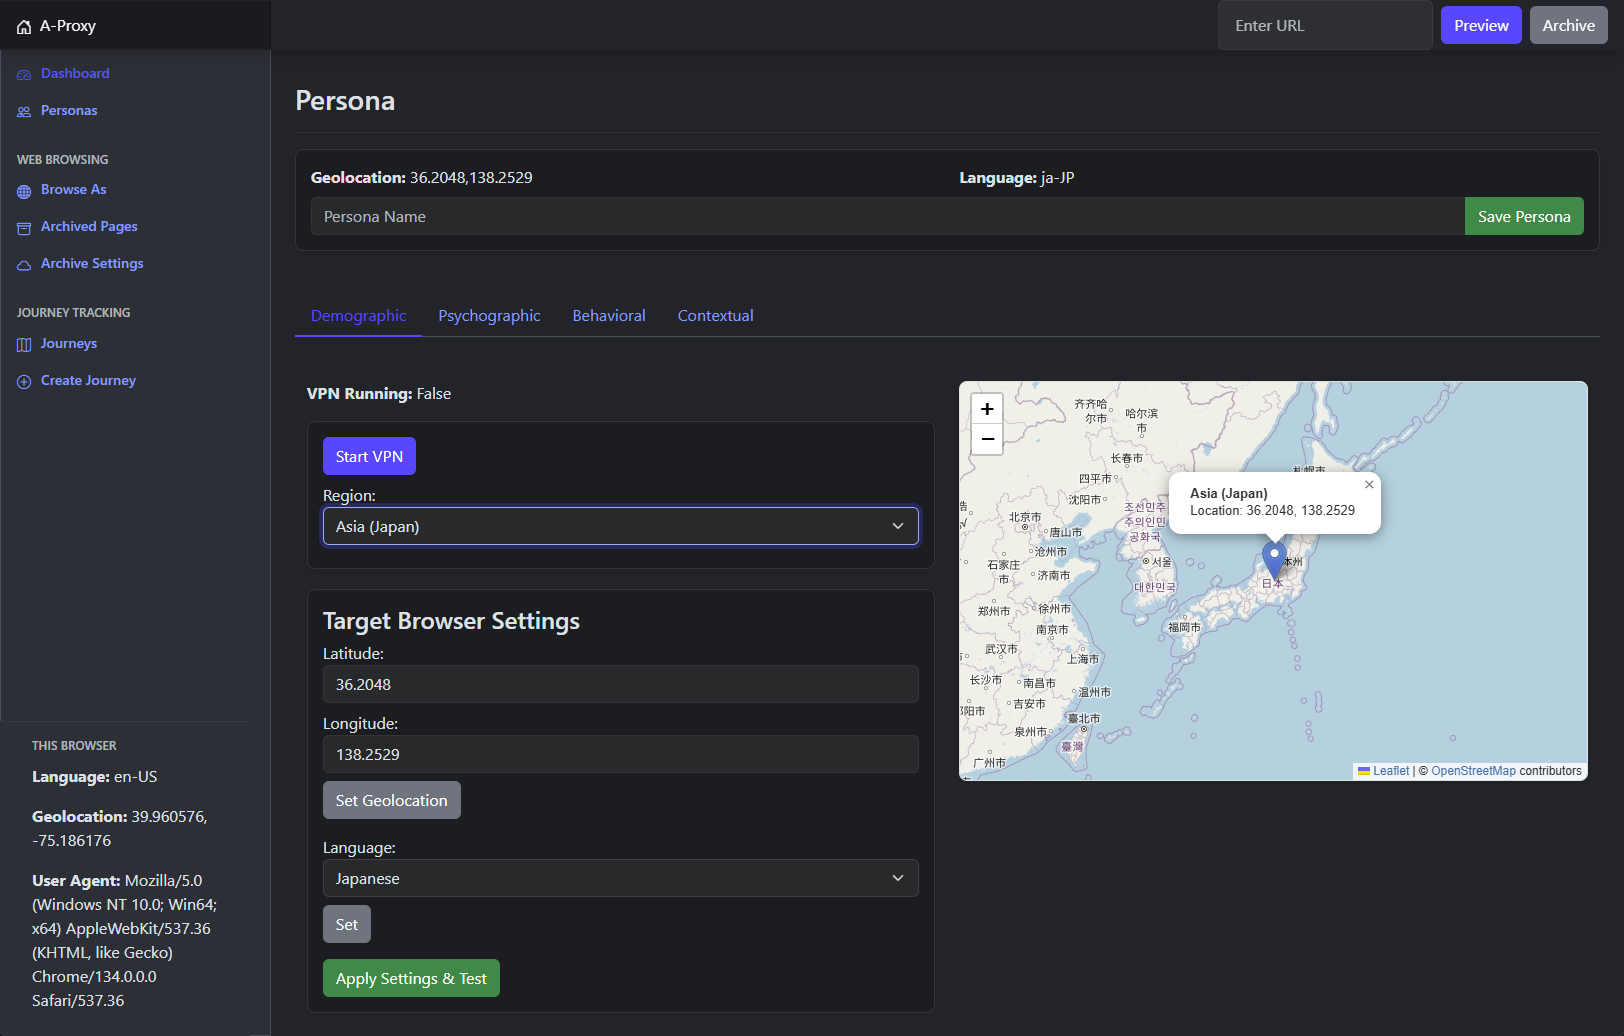
\includegraphics[width=.8\textwidth]{persona-teaser.png}
  \caption{Interface of the proxy system showing persona-level. See \url{https://youtu.be/FaQnB81BK6E}}
  \Description{Screenshot of A-Proxy interface showing persona settings, VPN toggle, and browser controls including geolocation and language.}
  \label{fig:persona}
\end{teaserfigure}
\maketitle


\section{Introduction}
This demo introduces A-Proxy, a tool designed to improve the fidelity of web archives by capturing and replaying personalized web browsing experiences. A preview video is available at \url{https://www.youtube.com/watch?v=FaQnB81BK6E}. 

Simulating the perspective of an individual user during web browsing and archiving presents significant challenges from both the technical and narrative perspectives. Personalized content varies according to location, language, and browsing habits. When pages are archived, these dynamic elements are often lost, making the original user experience difficult to reconstruct.

Kelly et al. (2013) \cite{kelly2013method} demonstrated that websites display varying content, such as news and weather, based on the GeoIP of a user or provided zip code. Sowbhagya et al. (2022) \cite{sowbhagya2022user} showed that integrating demographic data with behavioral insights produces more accurate user profiles in marketing contexts.
We propose adapting these marketing-based profiling techniques to improve web archiving. While marketers create detailed personas to target content delivery, archivists can leverage similar persona development to capture contextually relevant browsing experiences. By defining demographic characteristics, interests, and browsing patterns, much like how marketers segment their audiences, we can more faithfully record how web content adapts to different user profiles. This approach transforms traditional web archiving from capturing static content to preserving the dynamic, personalized nature of modern web experiences.

\section{Demo Scenario} The demonstration presents a scenario in which a simulated user profile is configured with demographic, behavioral, and contextual parameters, including geographic location via VPN. The system executes a browsing session that captures personalized content across several news and commerce websites. Captured data is stored in various formats, including screenshots, HTTP traffic, and WARC/WACZ files. It may be replayed using a web-based interface. Viewers can compare archived output generated by browsing as different personas and observe how the same page changes in response to user-specific variables. The video introductory demo and the tool repository are available at \url{https://www.youtube.com/watch?v=FaQnB81BK6E} and \url{https://github.com/savingads/a-proxy}, respectively.


\bibliographystyle{ACM-Reference-Format}
\bibliography{software}

\end{document}
